\begin{omgroup}[id=syntax-semantics]{Dimensions of Representation in \omdoc}
\begin{newpart}{re-read and strengthen the argumentation}
\begin{wrapfigure}r{8.5cm}\vspace*{-1em}
\fbox{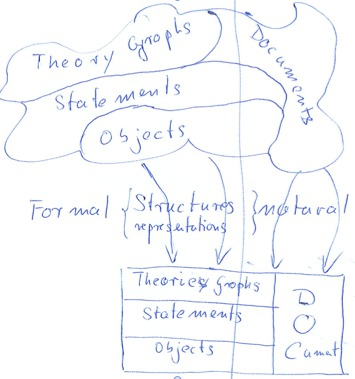
\includegraphics[width=8.2cm]{../figures/omdoc-dimensions}}
\caption{Dimensions of Representation in \omdoc}\label{fig:dimensions}\vspace*{-1em}
\end{wrapfigure}
\paragraph{Strict vs. Pragmatic} The \omdoc format is divided into two sub-languages:
``Strict'' \omdoc (in the lower half of Figure~\ref{fig:dimensions}) and ``Pragmatic''
\omdoc (in the upper half\ednote{add the words ``strict'' and ``pragmatic'' to the
  picture}). The first subset uses a minimal set of elements representing the meaning of a
mathematical expression in a uniform structure, while the second one tries to strike a
pragmatic balance between verbosity and formality. Both forms of content expressions are
legitimate and have their role in representing mathematics. The strict \omdoc format
features a minimal set of conceptually orthogonal representational primitives, resulting
in expressions with canonical structure, which simplifies the implementation of \omdoc
processors as well as the comparison of content expressions.  The pragmatic \omdoc
format provides a large representational infrastructure that aims at being intuitive for
humans to understand, read, and write.\ednote{maybe state the numbers of elements in the
  end} In particular, the simplicity and conceptual clarity of strict \omdoc allow to
express structural well-formedness constraints, whereas the vocabulary of pragmatic \omdoc
is much nearer to mathematical practice and is thus easier to learn. It is a crucial
design choice of the \omdoc format that the meaning fo pragmatic representations is
defined entirely interms of strict representations\footnote{The strategy of dividing a
  markup format into a simple and structurally elegant core language and a larger set of
  pragmatic extensions which can be given a meaning by translating into the core was first
  pioneered by the author for content {\mathml}3~\cite{CarlisleEd:MathML3}}. Note that
there may be multiple ``pragmatic vocabularies'' defined in terms of the strict core
catering to different communities and their tastes.

The introduction of strict \omdoc and the re-interpretation of pragmatic \omdoc in
terms of it is radical redesign of the \omdoc format, which is new in {\omdocv{1.6}}.
For this reason we consider {\omdocv{1.6}} the first step into the directiosn of
{\omdocv{2}}. With the development of strict \omdoc we aim to identify the
representational primitives for representing mathematical documents, which can be given a
simple and elegant semantics.

\paragraph{Formal vs. Informal} 

One of the hallmarks of mathematical language is that it is very rigorous in structure and
usage in an attempt to fix the meaning of (mathematical) objects and statements about
them. Indeed, the first decades of the last century established that mathematical language
can in principle be expanded into logical form, where all objects and statements are fully
identified by their syntactic form, and all reasoning steps are similarly justified by
their form alone. we speak of ``formal mathematics'', when this is exercised and of
``formal reasoning'', when proofs are carried out in logical systems on this basis . In
the last decades, significant parts of mathematical knowledge have been formalized and
verified with the help of computers. But formalization and formal reasoning is still so
costly and tedious that only a very small part of mathematics is formalized and verified
in practice. Currently almost all mathematical documents consist of a mix of formal and
informal (i.e. natural language) elements --- certainly during the development of
mathematical knowledge, but also in publications. Therefore representation formats for
mathematical documents must allow this as well, consequently, \omdoc has two
sub-languages, ``formal \omdoc'' (on the left side of Figure~\ref{fig:dimensions}) and
``natural \omdoc'' (on the right side).

\omdoc offers markup at three levels: objects, statements, and context.
\begin{compactdesc}
\item[objects] are usually represented as {\emph{formulae}} or \emph{natural language
    phrases} in mathematical documents. In formal \omdoc formulae are marked up according
  to their functional structure (as operator trees) and according to their layout in
  informal \omdoc (as layout trees). Note that any object can be represented in both ways
  and both ways of representation can be mixed at any level to account for mathematical
  practice, e.g. for mixed formulae like $\{n\in\mathbb{N}\bigl|\text{$n$ is prime and
    $n>2$}\}$.
\item[statements] are usually represented as \emph{natural language sentences (with
    formulae)}\footnote{or even larger text fragments made up of sentences like
    paragraphs} in informal settings and as (closed, logical) formulae in formal ones. The
  discussion about the two ways of representation of objects applies analogously. Note
  that functional markup in formal \omdoc only addresses part of the requirements of
  formality, since their meaning depends on their context; we will explore this next.
\item[theory graphs] The context of objects (and the statements that contain them) is
  given by special statements (declarations). For conciseness and tractability, \omdoc
  groups declarations into ``theories'' and connects them by ``theory morphisms'' into
  ``theory graphs''. In a nutshell, every object (and thus every statement) has a ``home
  theory'', in which it is meaningful. Theory morphisms make objects and statements
  available in their target theories.
\end{compactdesc}
As statements, theories and theory graphs are large objects, their informal
representations (as mathematical text fragments and documents) usually carry linguistic
cues to their discourse structure\ednote{change the ``documents'' in
  Figure~\ref{fig:dimensions} to ``discourse'', at least in the strict box}. We discuss
the relation between the discourse structure of informal representations and the formal
structure of statements and theory graphs next.

\paragraph{Discourse vs. Content Structure}

Mathematical documents are very explicitly structured to help the reader grasp the complex
objects, their relationships, and the flow of the argumentation in the proofs: Objects are
often represented as formulae that reveal their structure, statements are labeled by
indicators to their epistemic contribution to context (e.g. by labeling them as
``definitions'' or ``theorems'') and numbered for exact reference. The exposition of
larger documents usually follows a topical structure with superimposed narrative structure
driven by knowledge dependencies rather than e.g. a temporal dramaturgy driven by
suspense.  Even so, the structure of an informal document may be quite different from the
formal structure of the knowledge it introduces.

\begin{wrapfigure}l{7cm}\vspace*{-2em}
  \infigures{content_vs_narrative}
\caption{Content vs. Narrative Structures}\label{fig:straw-man}
\end{wrapfigure}
For instance, when we introduce a new concept in a course, we often first introduce a
naive reduced approximation $\mathcal{N}$ of the real theory $\mathcal{F}$, only to show
an example $\mathcal{E_N}$ of where this is insufficient. Then we propose a first
(straw-man) solution $\mathcal{S}$, and show an example $\mathcal{E_S}$ of why this does
not work. Based on the information we gleaned from this failed attempt, we build the
eventual version $\mathcal{F}$ of the concept or theory and demonstrate that this works on
$\mathcal{E_F}$.
 
The structure with the solid lines and boxes at the bottom of {\myfigref{straw-man}}
represents the content structure, where the circles $\mathcal{N}$, $\mathcal{E_N}$,
$\mathcal{S}$, $\mathcal{E_S}$, $\mathcal{F}$, and $\mathcal{E_F}$ signify theories for
the content of the respective concepts and examples. The arrows represent the
{\twintoo{theory}{inheritance}} structure, e.g. Theory $\mathcal{F}$ imports theory
$\mathcal{N}$. The top part of the diagram with the dashed lines stands for the narrative
structure, where the arrows mark up the document structure. For instance, the slides
$\text{sl}_i$ are grouped into a lecture. In the example in {\myfigref{straw-man}}, the
second slide of ``lecture'' presents the first example: the text fragment $\text{n}_1$
introduces it, and $\text{n}_2$ presents $\mathcal{E_N}$ and $\text{n}_2$ might say
something like ``this did not work in the current situation, so we have to extend the
conceptualization\ldots''. In a conventional setting, the narrative structure on the top
and the content structure would be represented in different documents: The lecture slides
and the formalization, and the equivalences (e.g. that $\text{n}_2$ verbalizes
$\mathcal{E_N}$; we have visualized these relations as dotted arrows in
{\myfigref{straw-man}}) could not be taken advantage of, since they are not explicitly
represented.

\begin{wrapfigure}r{7.5cm}\vspace*{-1em}
\infigures{adp}
\caption{The Active Documents Paradigm}\label{fig:adp}\vspace*{-1em}
\end{wrapfigure}
But these equivalences can be utilized to render services to the reader, for instance the
imports relation in the theory graph on the lower half of Figure~\ref{fig:straw-man}
induces a dependency relation that can be used to generate a minimal explanation (without
the motivation) of $\cE_\cF$.  For an example at the object level, consider for instance
the formula $a(x+y^2)$, whose layout is ambiguous in two places: $a$ could be a factor in
a product (presented as juxtaposition) or a function that is applied to an
argument. Likewise $y^2$ could be the variable $y$ raised to the second power or the
second element in the sequence $y^1,y^2,\ldots,y^n$. Humans can usually disambiguate this
from the context, but a screen reader service needs access to the operator tree to read
this as ``$a$ times [pause] $x$ plus $y$ squared'' or ``$a$ applied to [pause] $x$ plus
$y$ two''.

\omdoc aims to reconcile the dichotomy between discourse structures (in informal
mathematical documents which currently carry most of mathematical knowledge) and formal
structures (that machines can operate upon) in one joint format. The central technique
employed in \omdoc is that of ``parallel markup'': The technique comes from MathML, where
the \element{semantics} element is used to accomodate equivalent layout (presentation
{\mathml}) and operator trees (content {\mathml}) and possibly foreign
representations. Equivalence of nested sub-structures are represented by special
cross-references.  The \mathml processor choses the one most adequate to its task --- in
the absence of distinguisthing information the first child.

\omdoc extends this to the document level: The document contains elements whose children
are alternative representations of the same object/statement/theory.\ednote{implement
  this, and think about the cross-referencing, also need continuations to break tree
  overlaps, e.g. in content objects straddling slides.} The significance of this is

for that is Figure~\ref{fig:adp} shows the \ednote{talk about parallel markup, content
  documents and narrative documents and how to crosslink them and share structure}.


Just as for content-based systems on the formula level, there are now MKM systems that
generate presentation markup from content markup, based on general presentation
principles, also on this level. For instance, the {\sc{ActiveMath}}
system~\cite{MelBue:krma03} generates a simple narrative structure (the
presentation; called a personalized book) from the underlying content structure (given in
\omdoc) and a user model.

\paragraph{Coverage} 
Currently our understanding of these primitives is largely limited to formal parts of
mathematics, therefore strict {\omdocv{1.6}} covers significantly less of informal
mathematical documents than {\omdocv{1.2}}, so the meaning-giving translation from
pragmatic \omdoc elements to strict \omdoc is partial. We plan to develop strict
\omdoc into a system with greater coverage in the upcoming versions of \omdoc.
{\omdocv{2.0}} will be the first stable version where the coverage of strict \omdoc is
complete.
\end{newpart}
\end{omgroup}

%%% Local Variables:
%%% mode: latex
%%% TeX-master: t
%%% End:
